\begin{auf}
    686.5
\end{auf}
Am Ende einer horizontal angeordneten Feder befindet sich eine Metallplatte von $m=0.1kg$ Masse. Die Feder wird, ausgehend von ihrer entspannten Ruhelage (1), um $x_m=5cm$ zusammengedrückt (2) und danach losgelassen. Reibung und die Gewichtskraft von $m$ werden vernachlässigt.
\begin{enumerate}
    \item[a] Wie lautet die Bewegungsgleichung (Differenzialgleichung) für die Masse $m$?
    \item[b] Wie groß ist die Federkonstante $k$, wenn die Platte harmonische Schwingungen mit der Periodendauer $T=0.5s$ ausführt?
    \item[c] Welche maximale Geschwindigkeit $v_m$ und maximale Beschleunigung $a_m$ erreicht die Platte	während der Schwingungen?
    \item[d] Skizzieren Sie die $x(t)$-, $v(t)$- und $a(t)$-Diagramme!
\end{enumerate}
\begin{figure}[h]
    \centering
    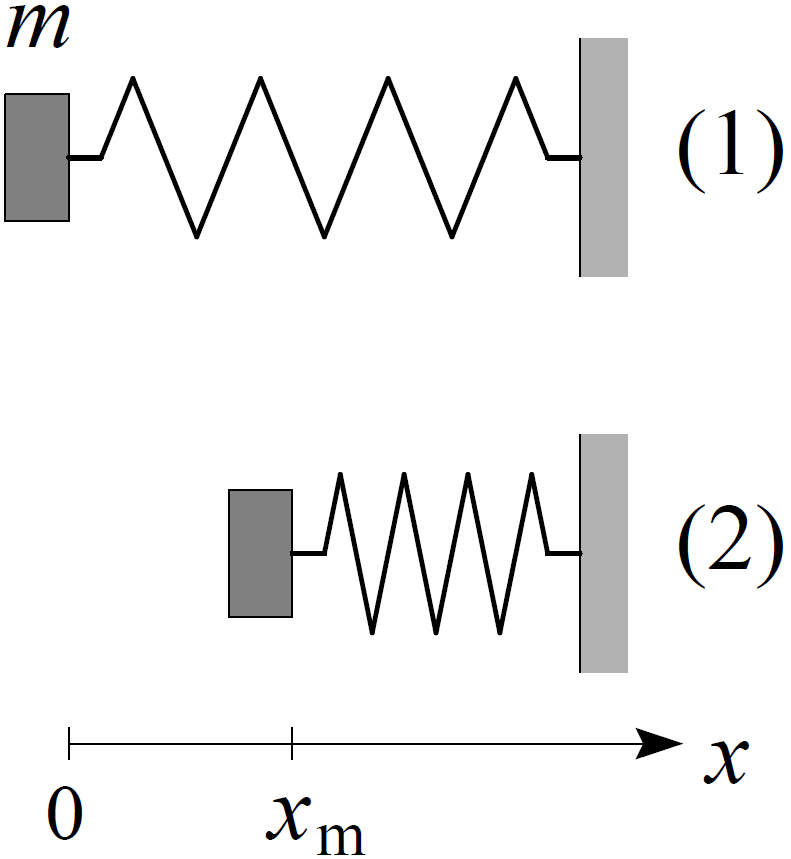
\includegraphics[height=5cm]{images/686,5_0.png}
    \caption{Versuchsaufbau Aufgabe 686.5}
\end{figure}